\documentclass[]{scrartcl}

\usepackage{geometry}
 \geometry{
 a4paper,
 total={170mm,257mm},
 left=20mm,
 top=20mm,
 }

\usepackage{multirow}
\usepackage{pdflscape}
\usepackage{graphicx}

%opening
\title{VSL graphics}
\author{}

\begin{document}

\maketitle

\begin{abstract}

\end{abstract}

\section{Asia network}

Configuration for \textbf{asia}:

\begin{itemize}
\item number of nodes: 8
\item number of arcs: 8
\item number of parameters: 18
\item average degree: 2
\item maximum in-degree: 2
\item number of samples of train dataset: 100
\item number of samples of test dataset: 10000
\item number of iterations: 140
\item parent sets size: \{100\}
\end{itemize}

Summary data:

\begin{itemize}
\item map train:  $-223.48  \pm  9.45$
\item map test:  $-198.38  \pm  3.77$
\item bma train:  $-196.18  \pm  9.32$
\item bma test:  $-199.56  \pm  11.07$
\item bnlearn train:  $-254.26  \pm  7.62$
\item bnlearn test:  $-233.82  \pm  3.87$
\end{itemize}

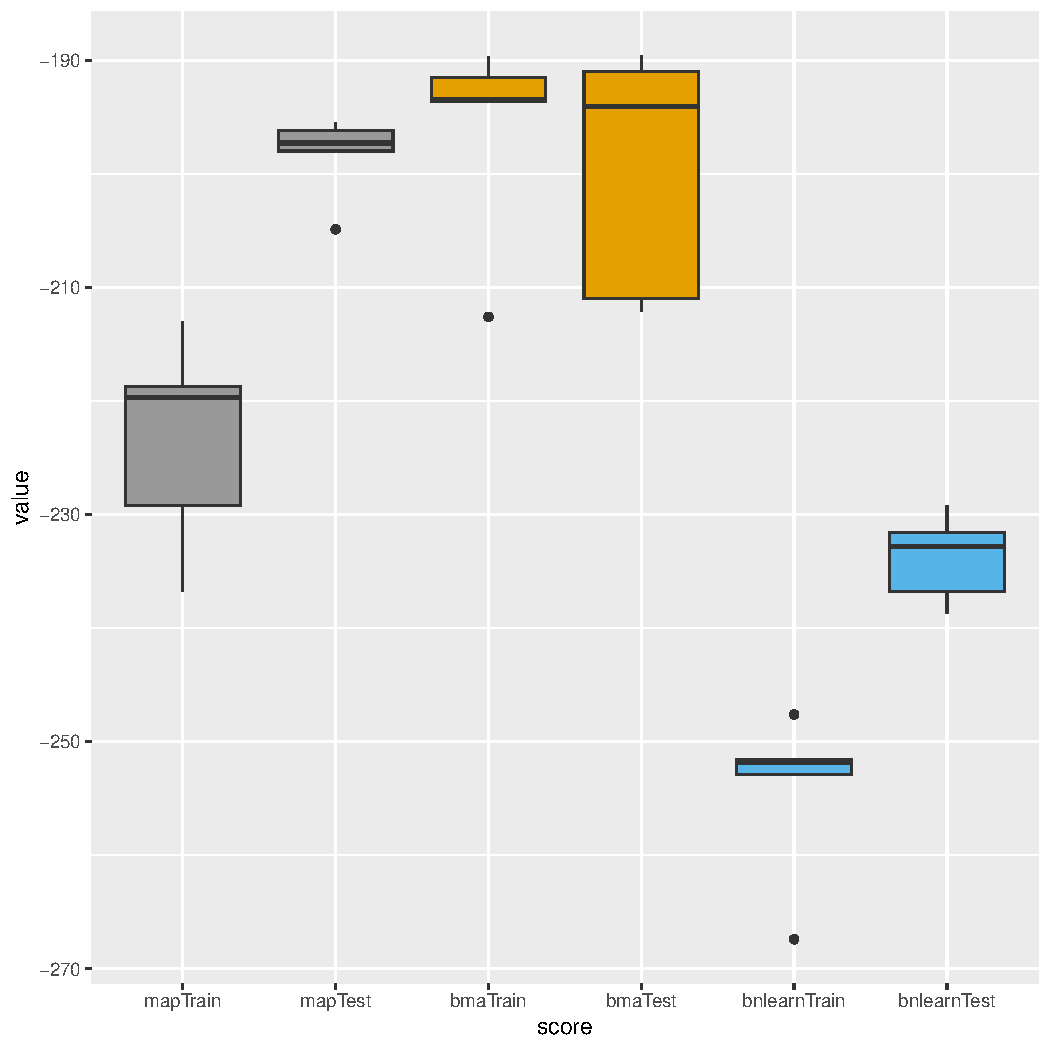
\includegraphics[scale = 0.5]{./figs/asia/asia-boxplots.pdf}

\subsection{Graphics of evolution}

\begin{tabular}{cc}
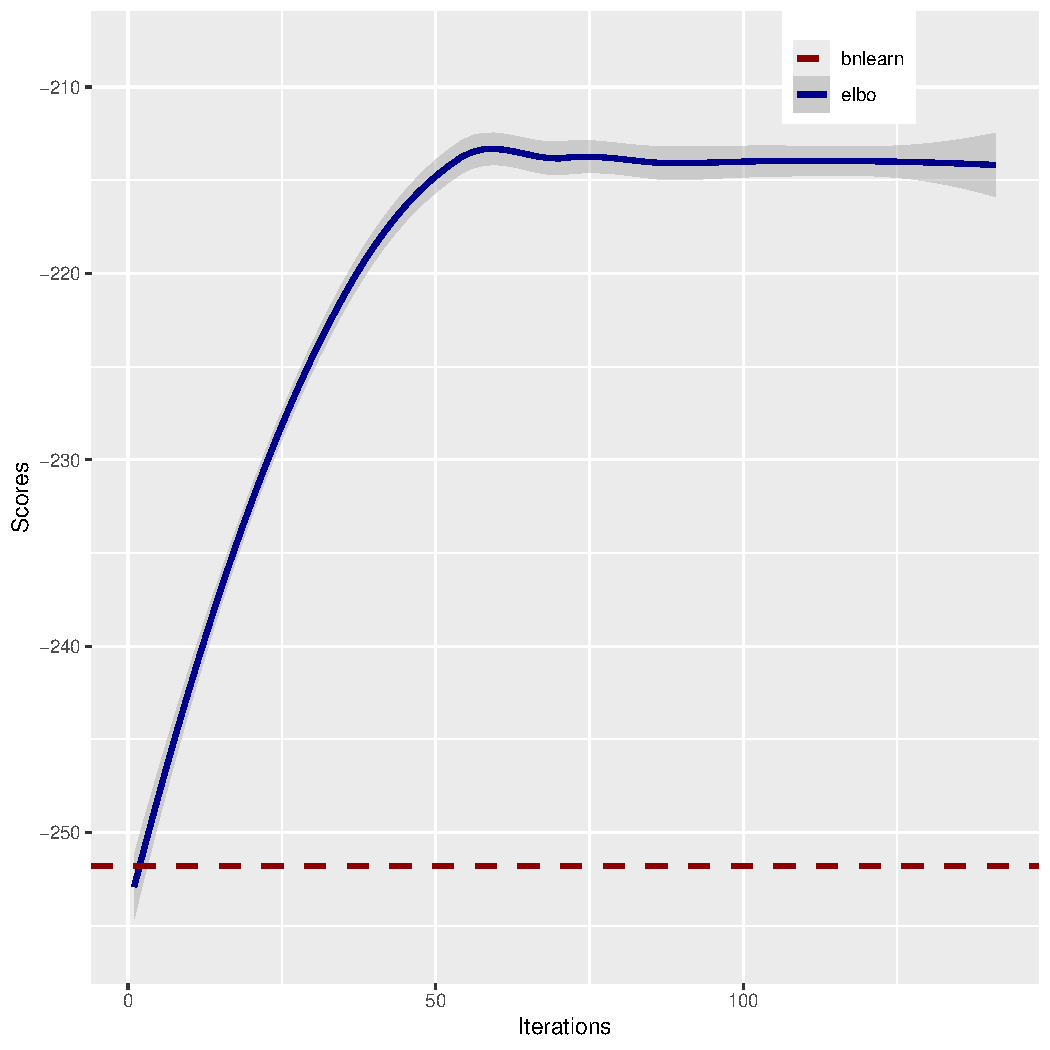
\includegraphics[scale = 0.4]{./figs/asia/mapEvolution-1-142.pdf} &
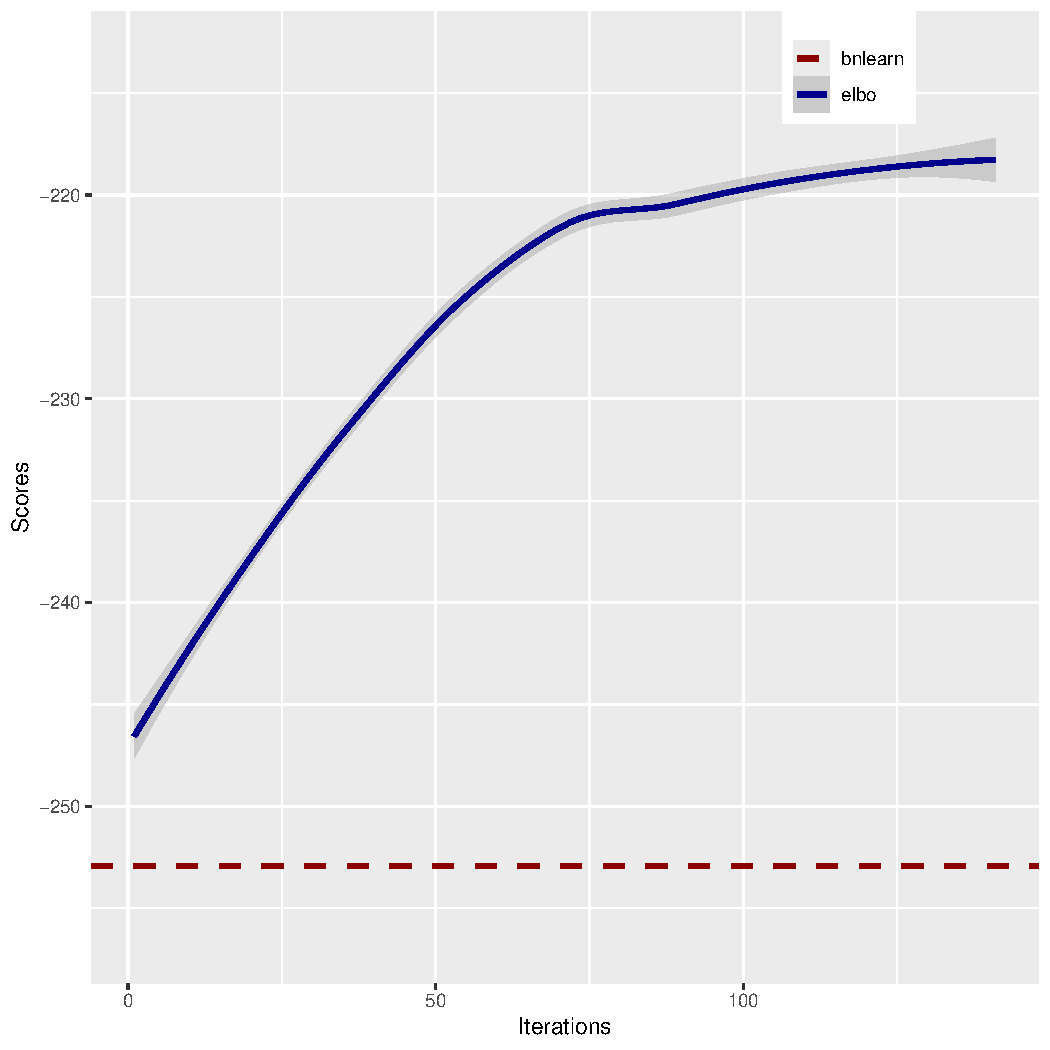
\includegraphics[scale = 0.4]{./figs/asia/mapEvolution-2-142.pdf} \\
\end{tabular}

\begin{tabular}{cc}
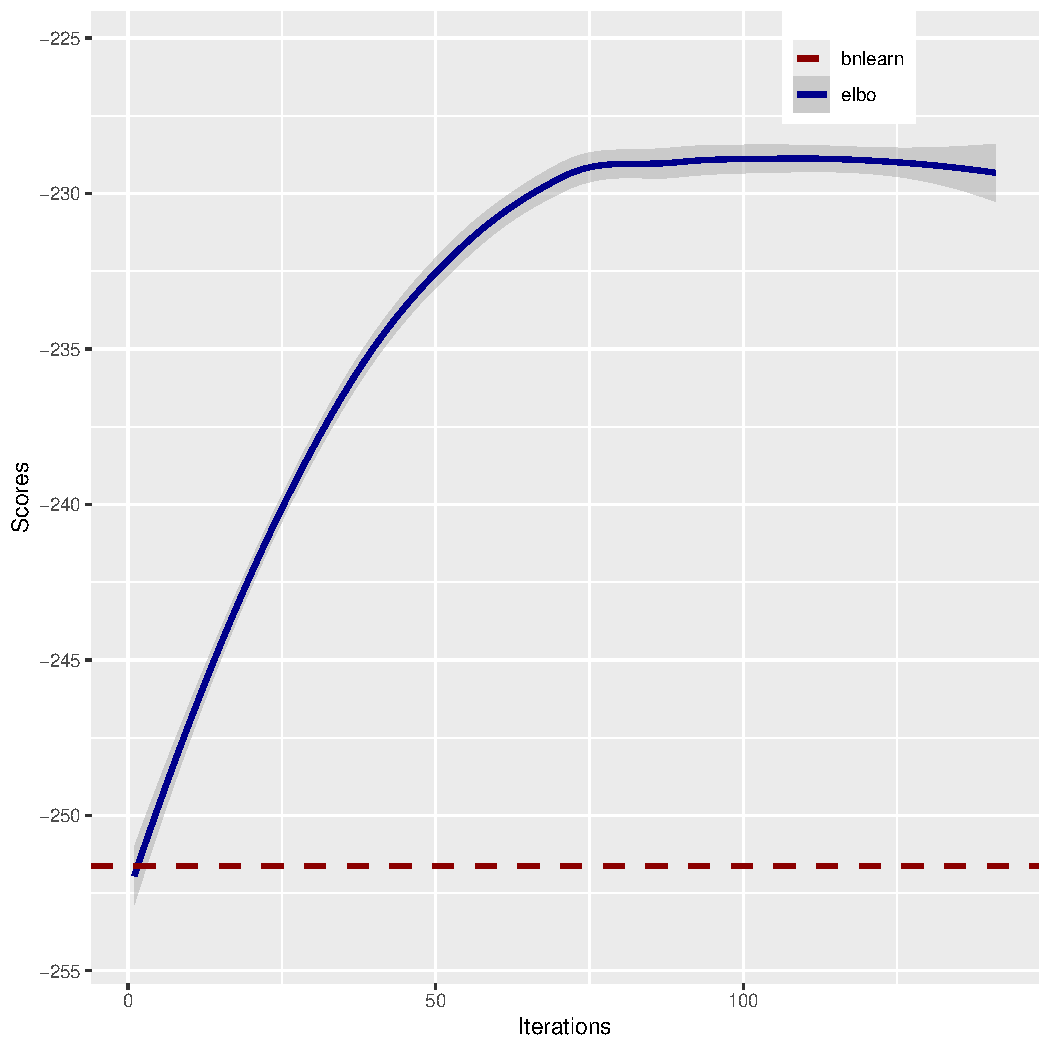
\includegraphics[scale = 0.4]{./figs/asia/mapEvolution-3-142.pdf} &
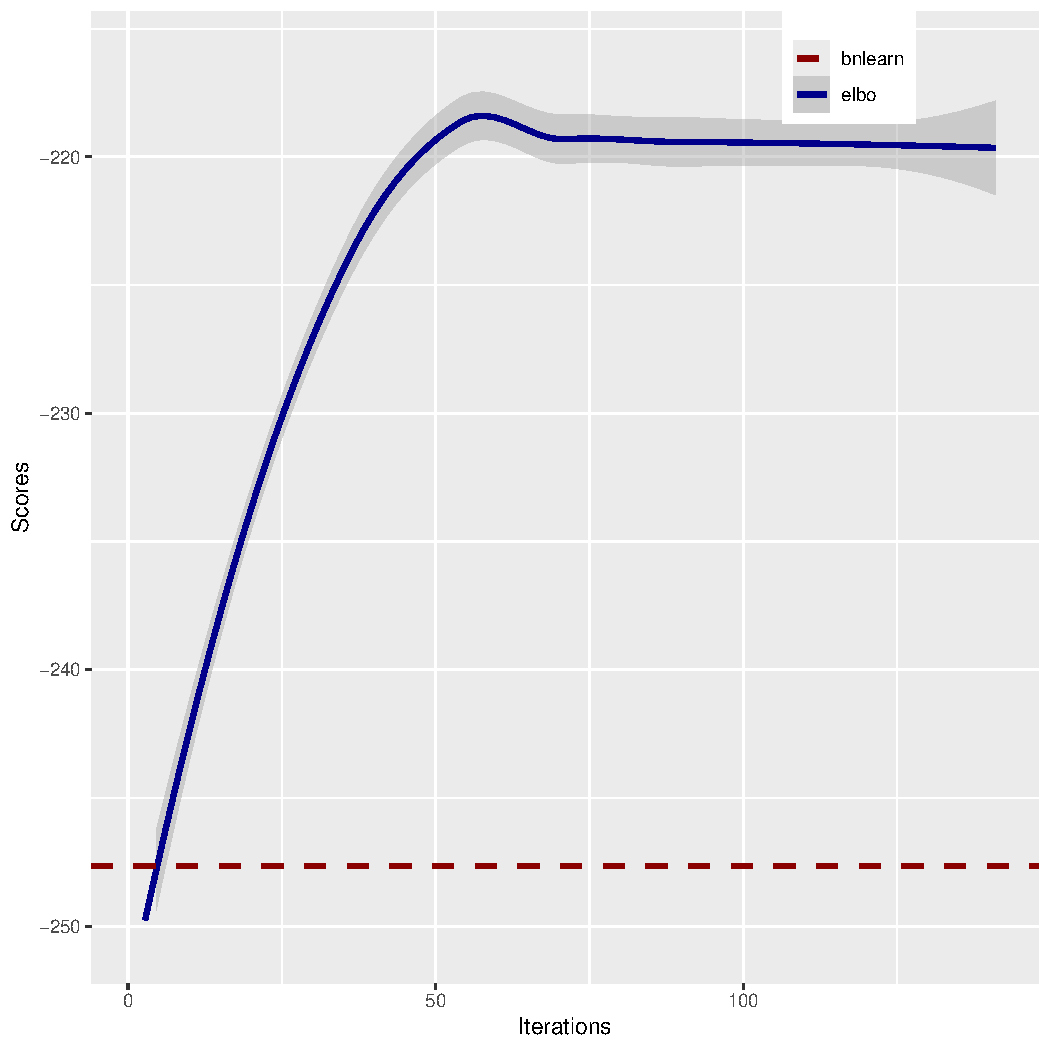
\includegraphics[scale = 0.4]{./figs/asia/mapEvolution-4-142.pdf} \\
\end{tabular}

\begin{tabular}{cc}
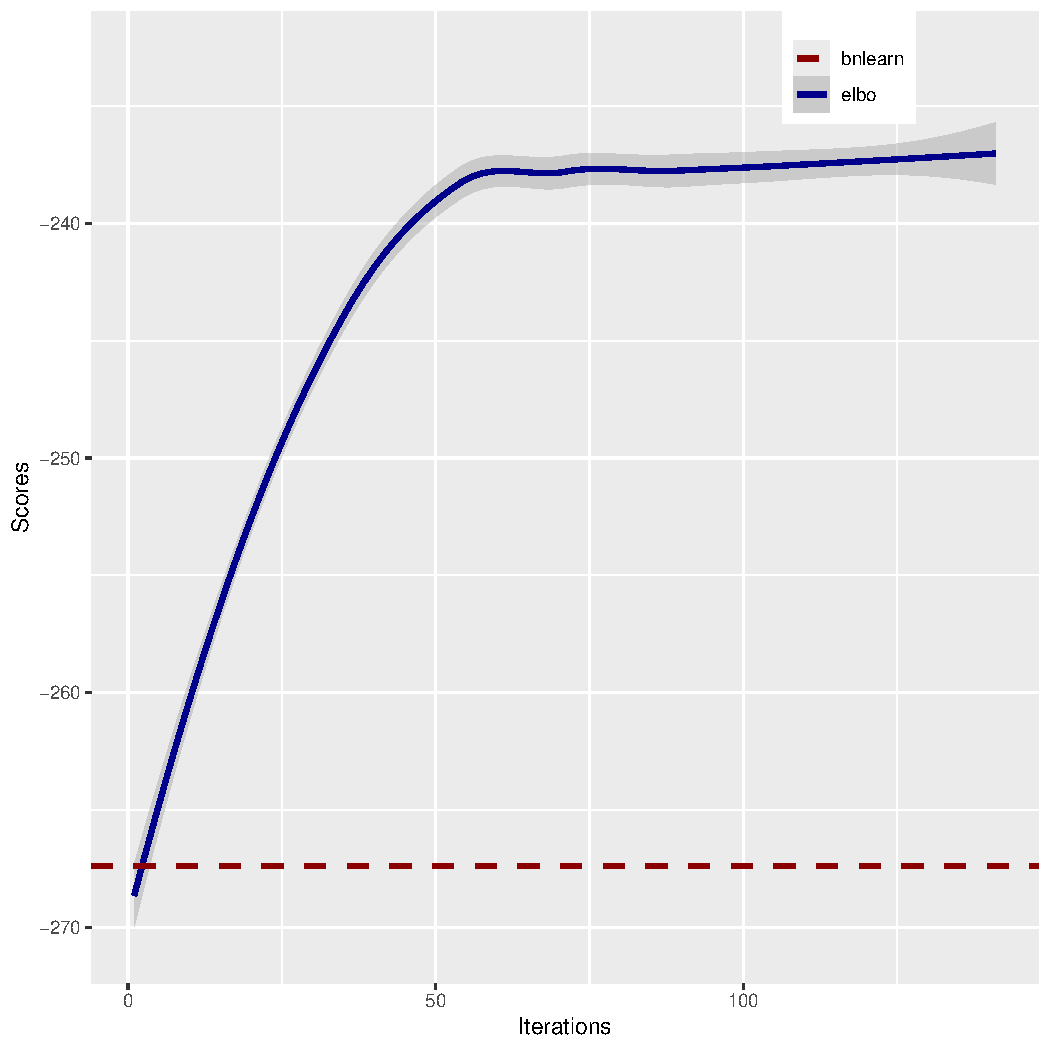
\includegraphics[scale = 0.4]{./figs/asia/mapEvolution-5-142.pdf}  & \\
\end{tabular}

\clearpage

\section{Alarm network}

Configuration for \textbf{alarm}:

\begin{itemize}
\item number of nodes: 37
\item number of arcs: 46
\item number of parameters: 509
\item average degree: 2.49
\item maximum in-degree: 4
\item number of samples of train dataset: 600
\item number of samples of test dataset: 10000
\item number of iterations: 3330
\item parent sets size: \{100\}
\end{itemize}

Summary data:

\begin{itemize}
\item map train:  $-5719.40  \pm  86.26$
\item map test:  $-5233.80  \pm  60.67$
\item bma train:  $-5189.80  \pm  63.77$
\item bma test:  $-5189.60  \pm  61.30$
\item bnlearn train:  $-6980.60  \pm  76.64$
\item bnlearn test:  $-6663.20  \pm  89.17$
\end{itemize}

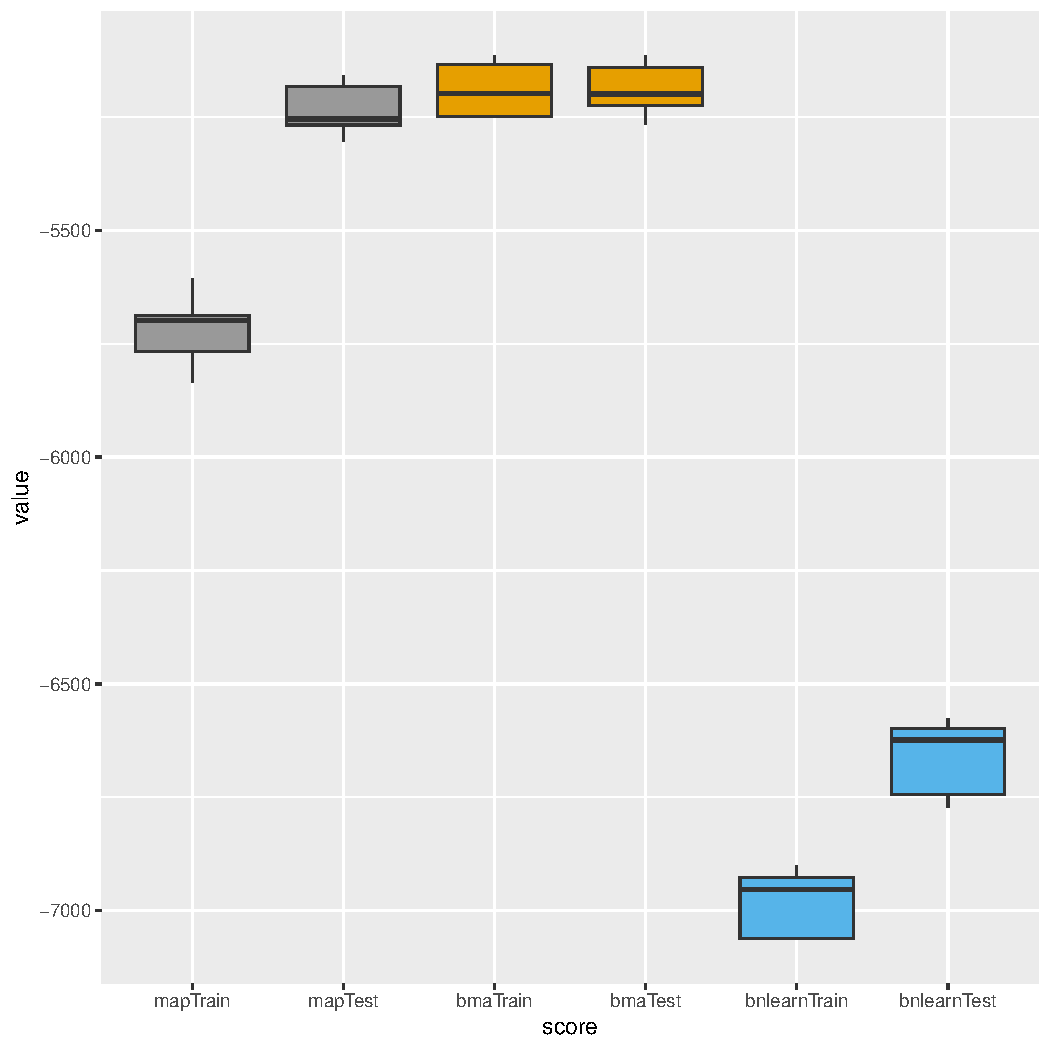
\includegraphics[scale = 0.5]{./figs/alarm/alarm-boxplots.pdf}

\subsection{Graphics of evolution}

\begin{tabular}{cc}
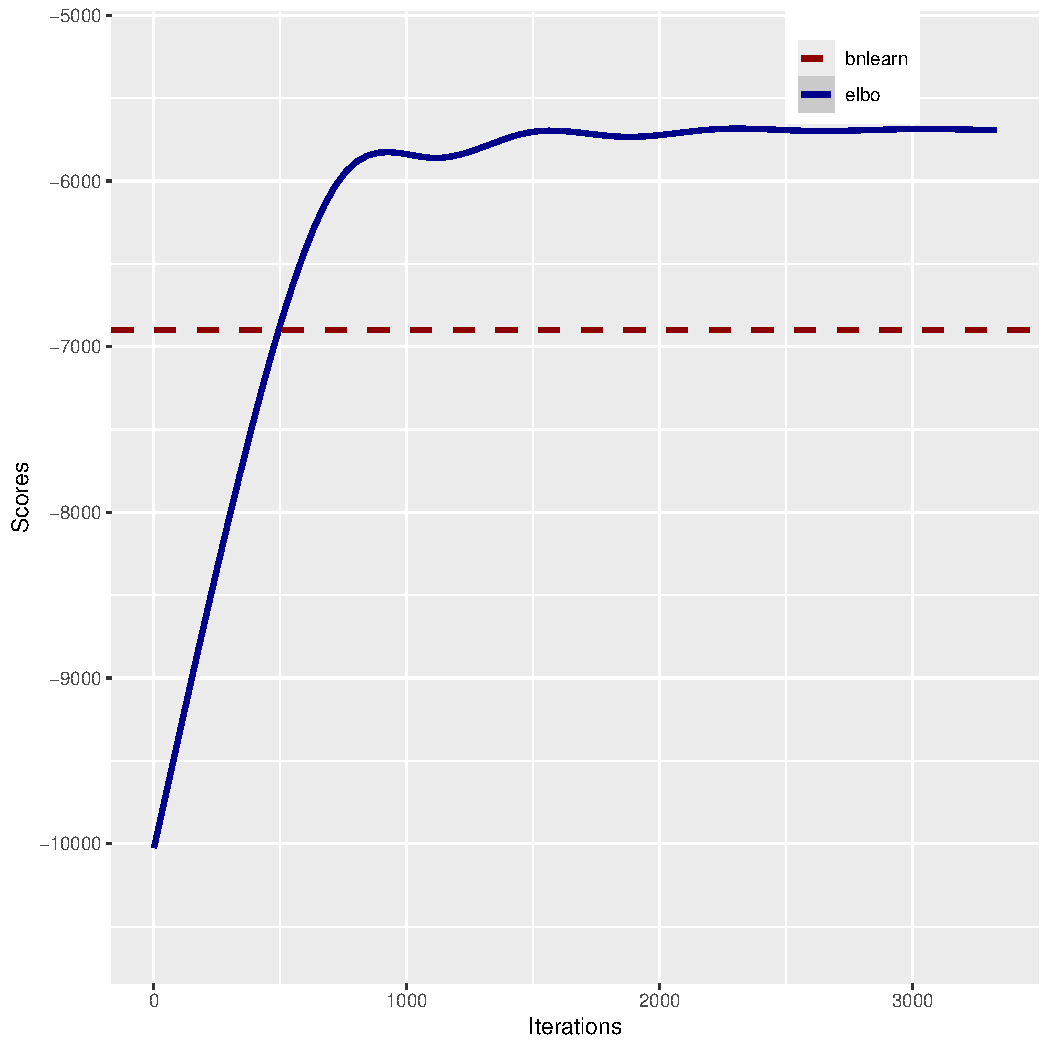
\includegraphics[scale = 0.4]{./figs/alarm/mapEvolution-1-3332.pdf} &
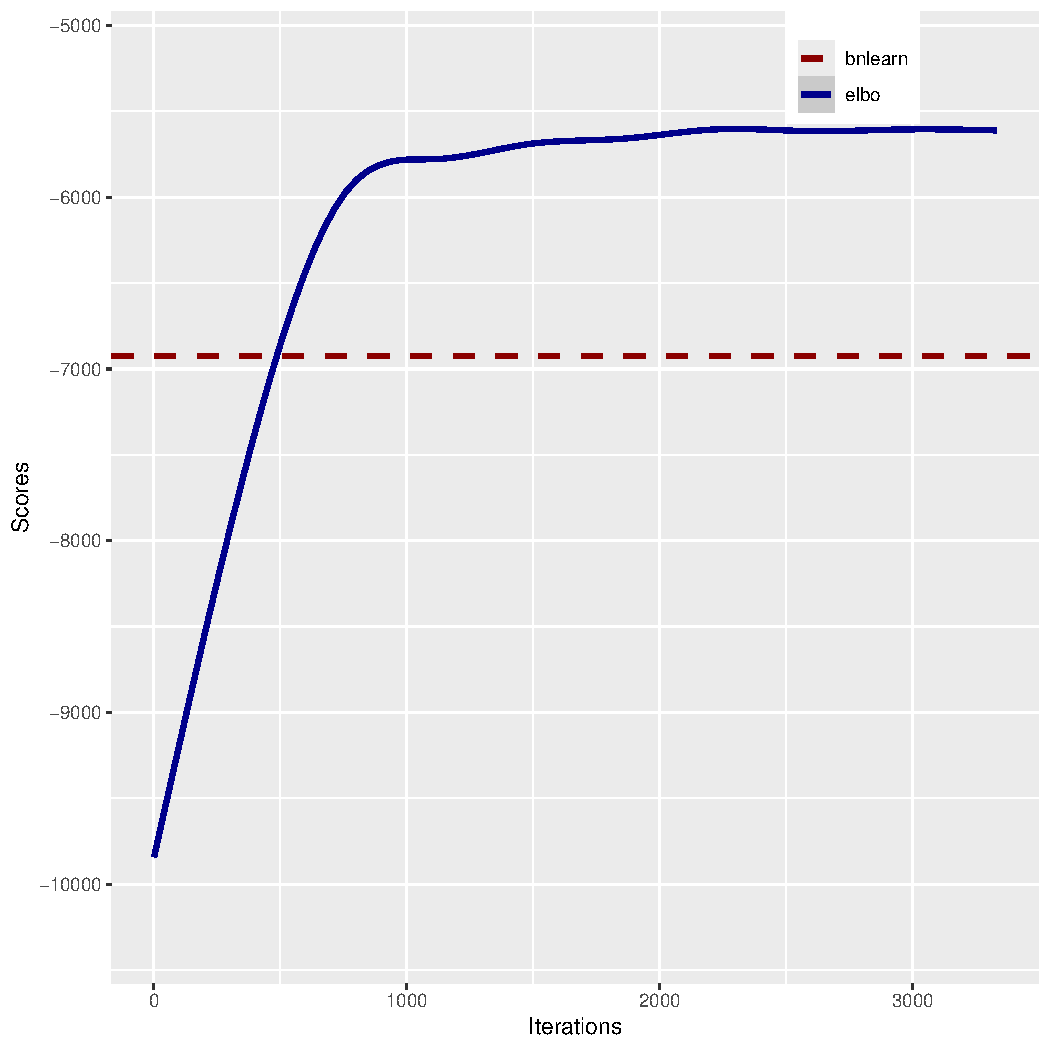
\includegraphics[scale = 0.4]{./figs/alarm/mapEvolution-2-3332.pdf} \\
\end{tabular}

\begin{tabular}{cc}
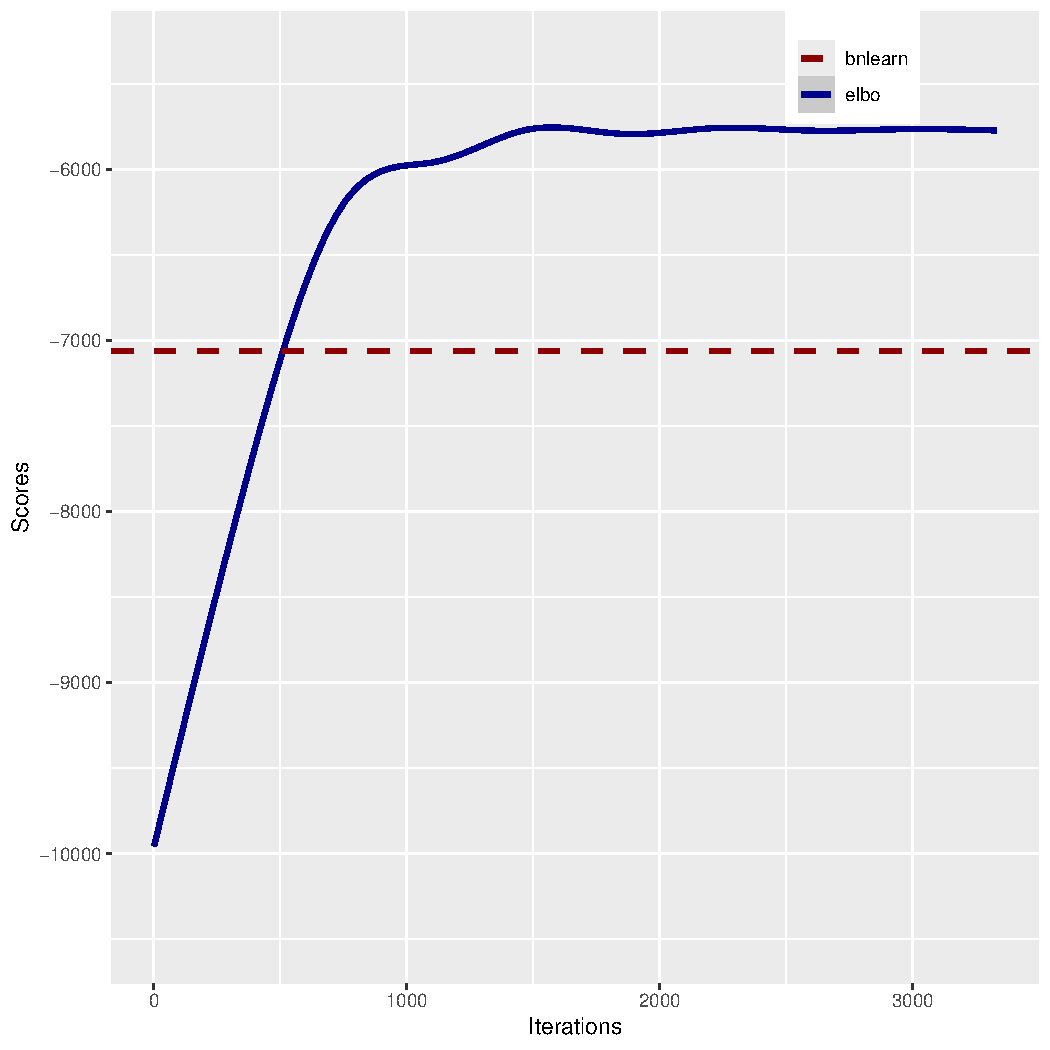
\includegraphics[scale = 0.4]{./figs/alarm/mapEvolution-3-3332.pdf} &
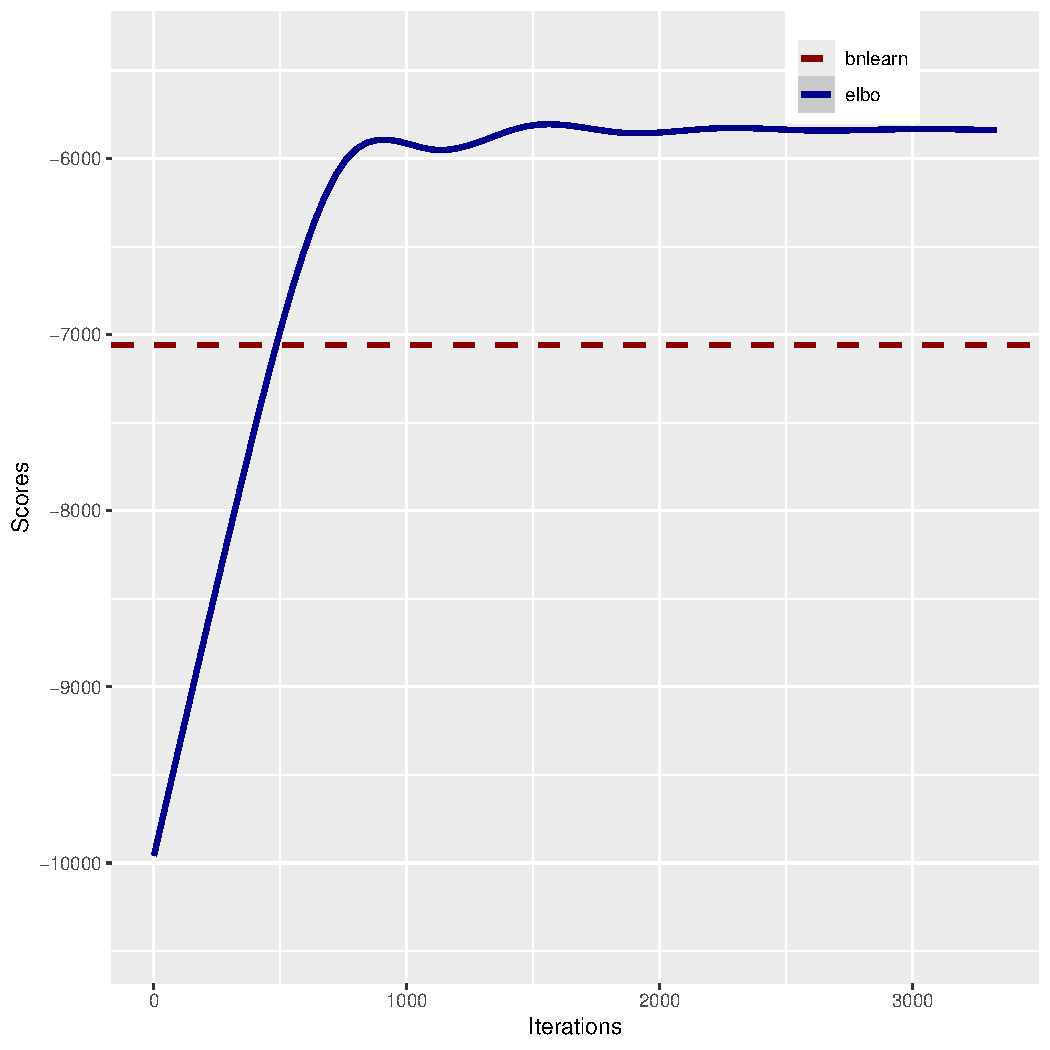
\includegraphics[scale = 0.4]{./figs/alarm/mapEvolution-4-3332.pdf} \\
\end{tabular}

\begin{tabular}{cc}
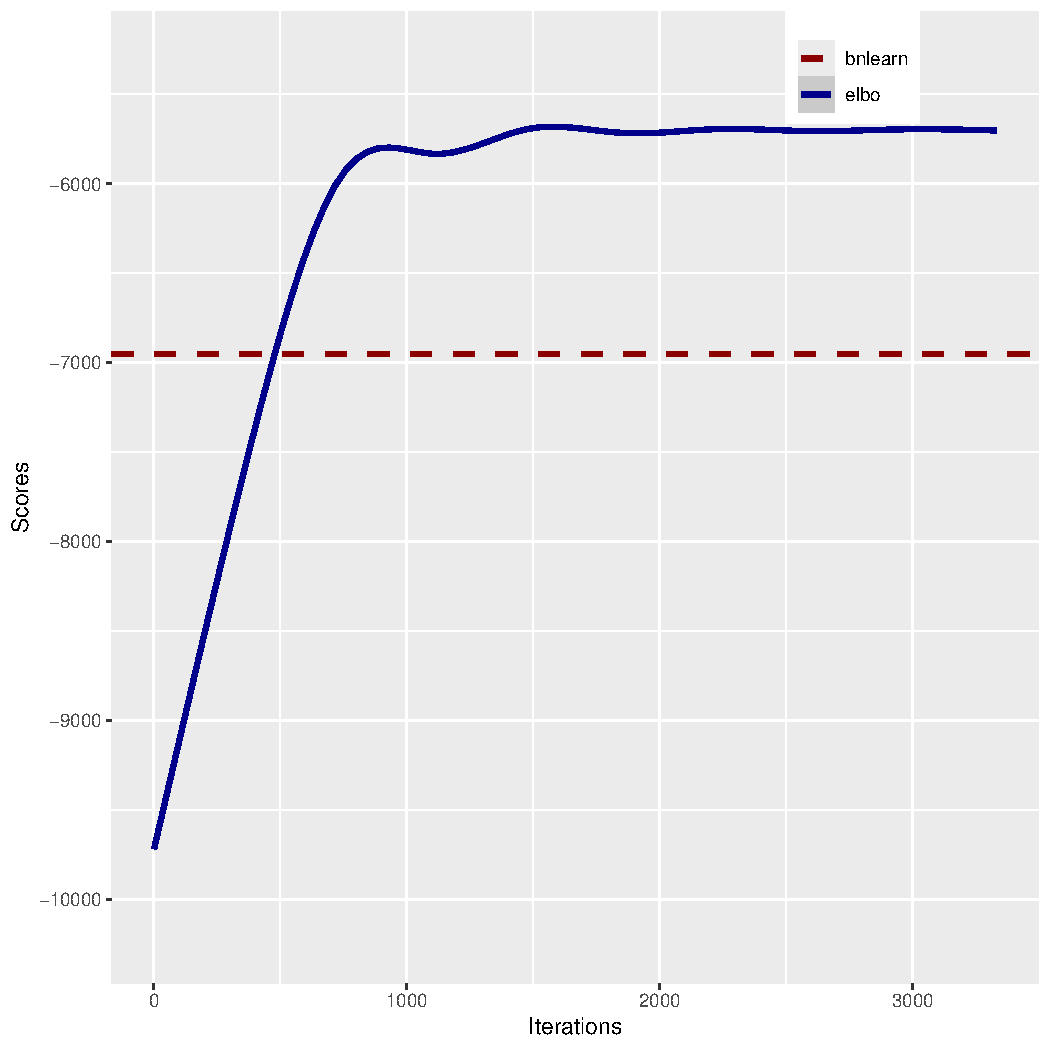
\includegraphics[scale = 0.4]{./figs/alarm/mapEvolution-5-3332.pdf} & \\
\end{tabular}

\clearpage

\section{Hepar2}

Configuration for \textbf{hepar2}:

\begin{itemize}
\item number of nodes: 70
\item number of arcs: 123
\item number of parameters: 1453
\item average degree: 3.51
\item maximum in-degree: 6
\item number of samples of train dataset: 3000
\item number of samples of test dataset: 10000
\item number of iterations: 12075
\item parent sets size: \{100\}
\end{itemize}

Summary data:

\begin{itemize}
\item map train:  $-98121.80  \pm  200.92$
\item map test:  $-97686.00  \pm  53.89$
\item bma train:  $-97513.80  \pm  147.95$
\item bma test:  $-97523.60  \pm  116.64$
\item bnlearn train:  $-98506.80  \pm  190.09$
\item bnlearn test:  $-98124.20  \pm  13.90$
\end{itemize}

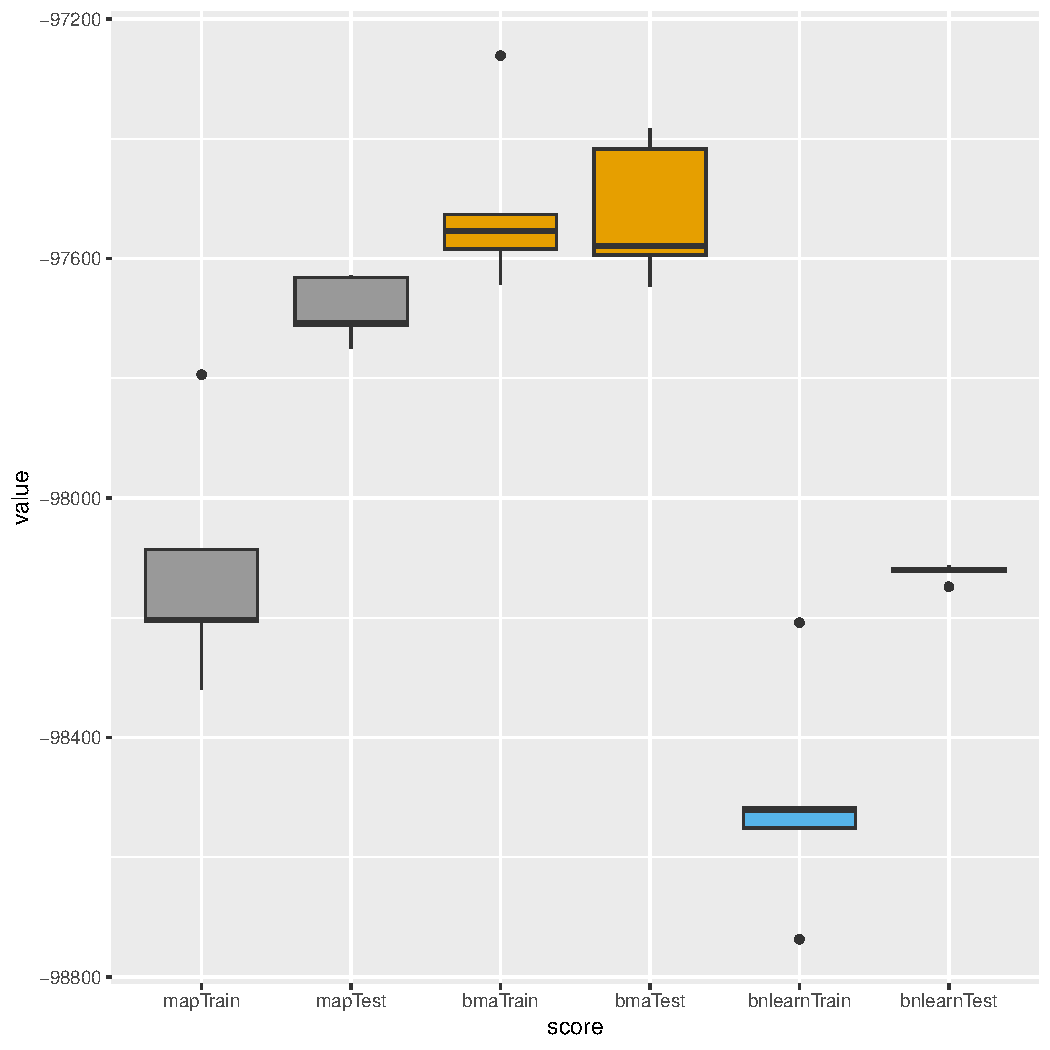
\includegraphics[scale = 0.5]{./figs/hepar2/hepar2-boxplots.pdf}

\subsection{Graphics of evolution}

\begin{tabular}{cc}
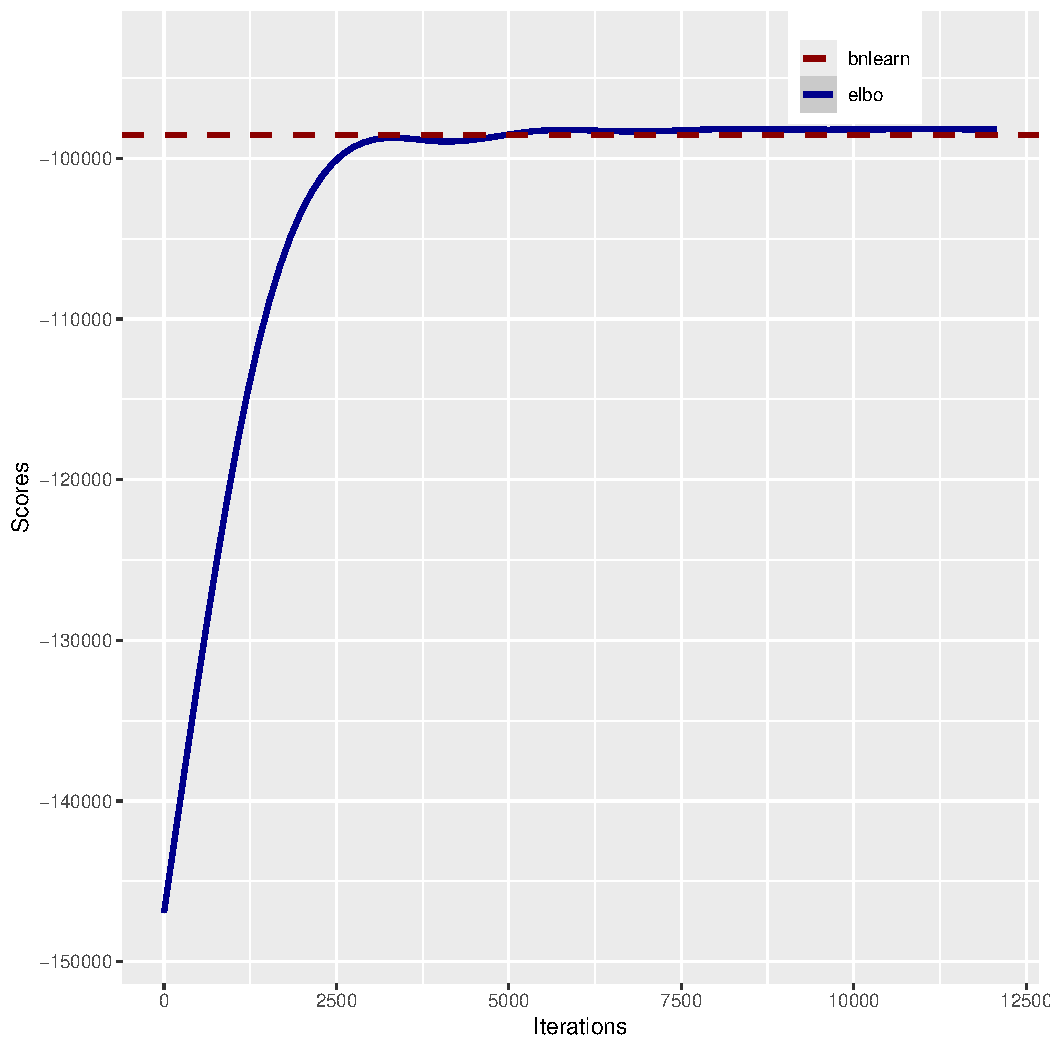
\includegraphics[scale = 0.4]{./figs/hepar2/mapEvolution-1-12077.pdf} &
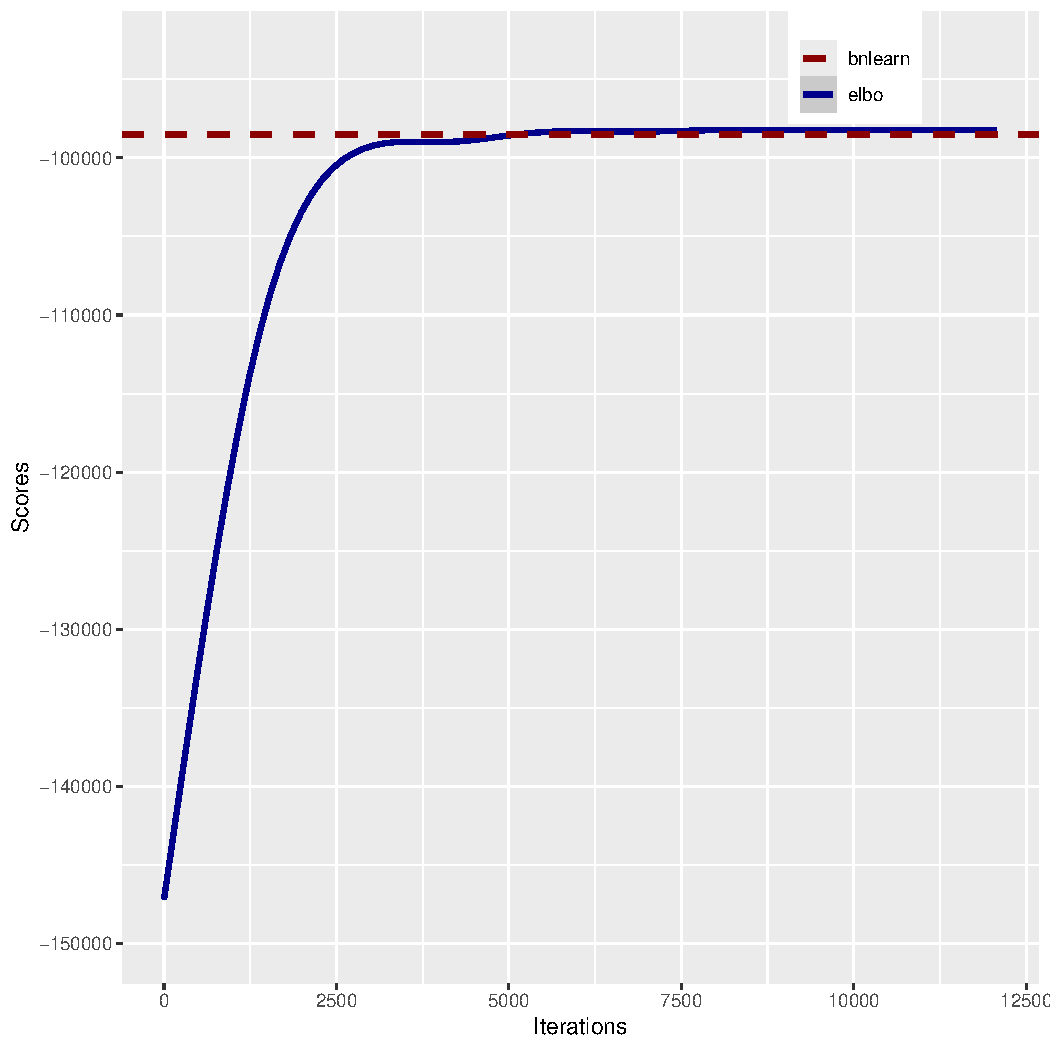
\includegraphics[scale = 0.4]{./figs/hepar2/mapEvolution-2-12077.pdf} \\
\end{tabular}

\begin{tabular}{cc}
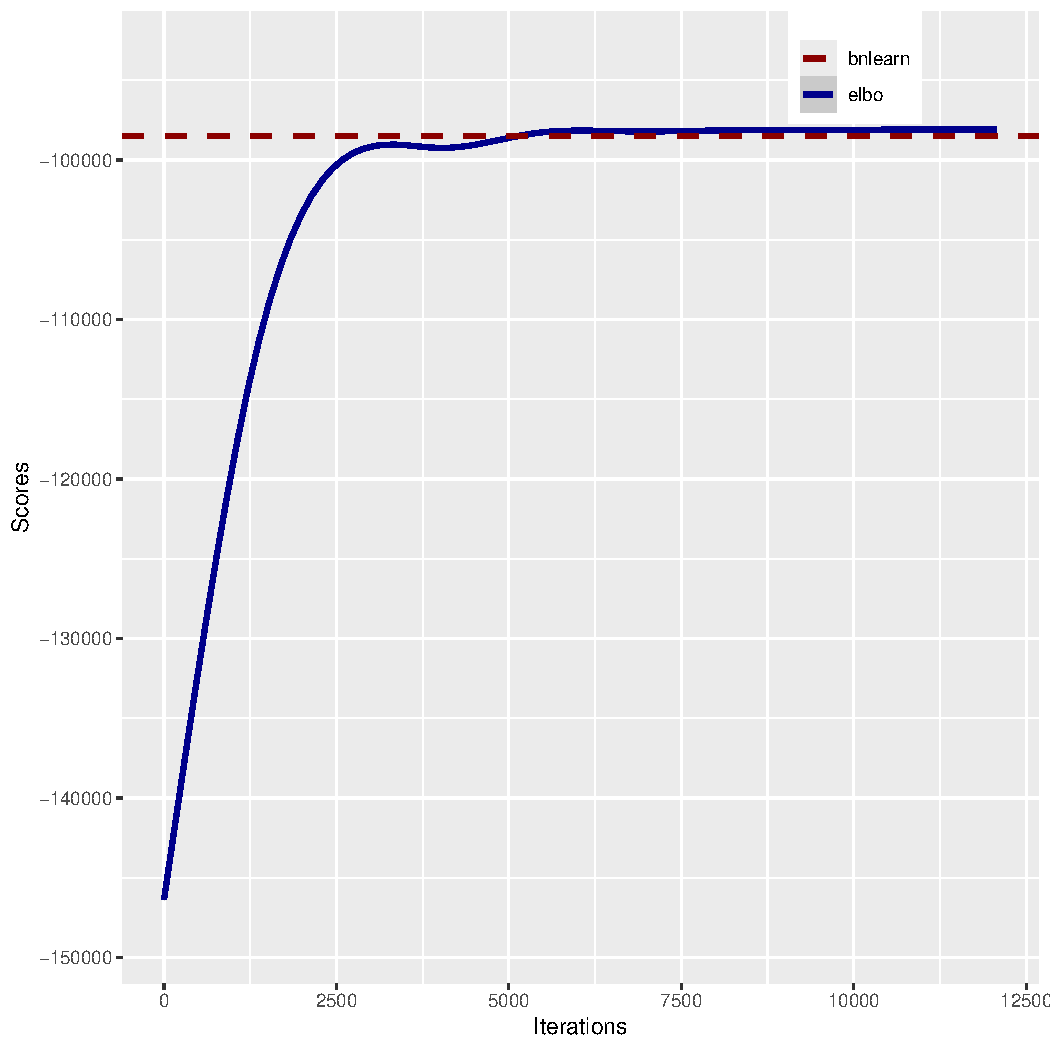
\includegraphics[scale = 0.4]{./figs/hepar2/mapEvolution-3-12077.pdf} &
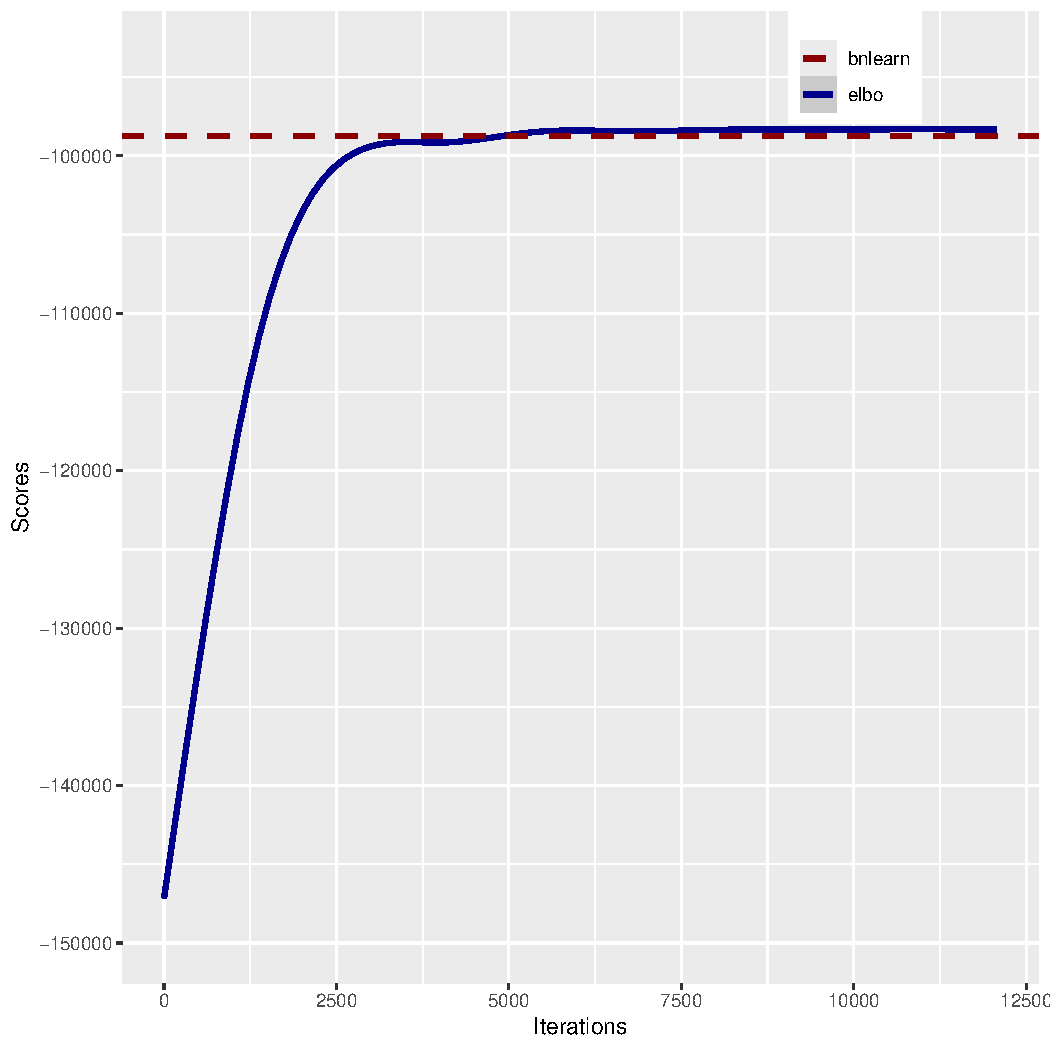
\includegraphics[scale = 0.4]{./figs/hepar2/mapEvolution-4-12077.pdf} \\
\end{tabular}

\begin{tabular}{cc}
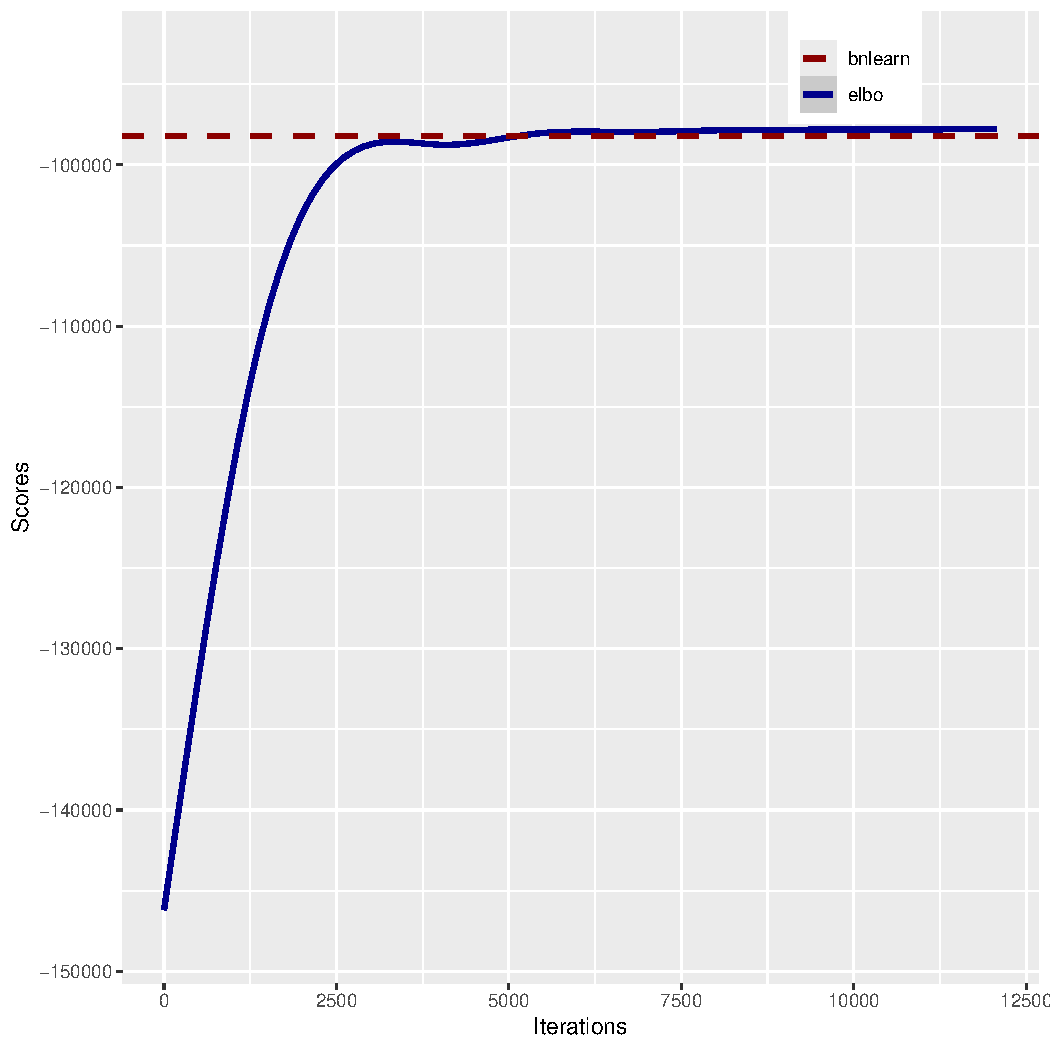
\includegraphics[scale = 0.4]{./figs/hepar2/mapEvolution-5-12077.pdf} &  \\
\end{tabular}


\section{Win95pts}

Configuration for \textbf{win95pts}:

\begin{itemize}
\item number of nodes: 76
\item number of arcs: 112
\item number of parameters: 574
\item average degree: 2.95
\item maximum in-degree: 7
\item number of samples of train dataset: 2500
\item number of samples of test dataset: 10000
\item number of iterations: 14250
\item parent sets size: \{100\}
\end{itemize}


Summary data:

\begin{itemize}
\item map train:  $-16576.40  \pm  75.91$
\item map test:  $-15991.40  \pm  55.58$
\item bma train:  $-16165.40  \pm  67.25$
\item bma test:  $-16156.00  \pm  46.21$
\item bnlearn train:  $-23436.40  \pm  100.75$
\item bnlearn test:  $-23167.00  \pm  123.16$
\end{itemize}

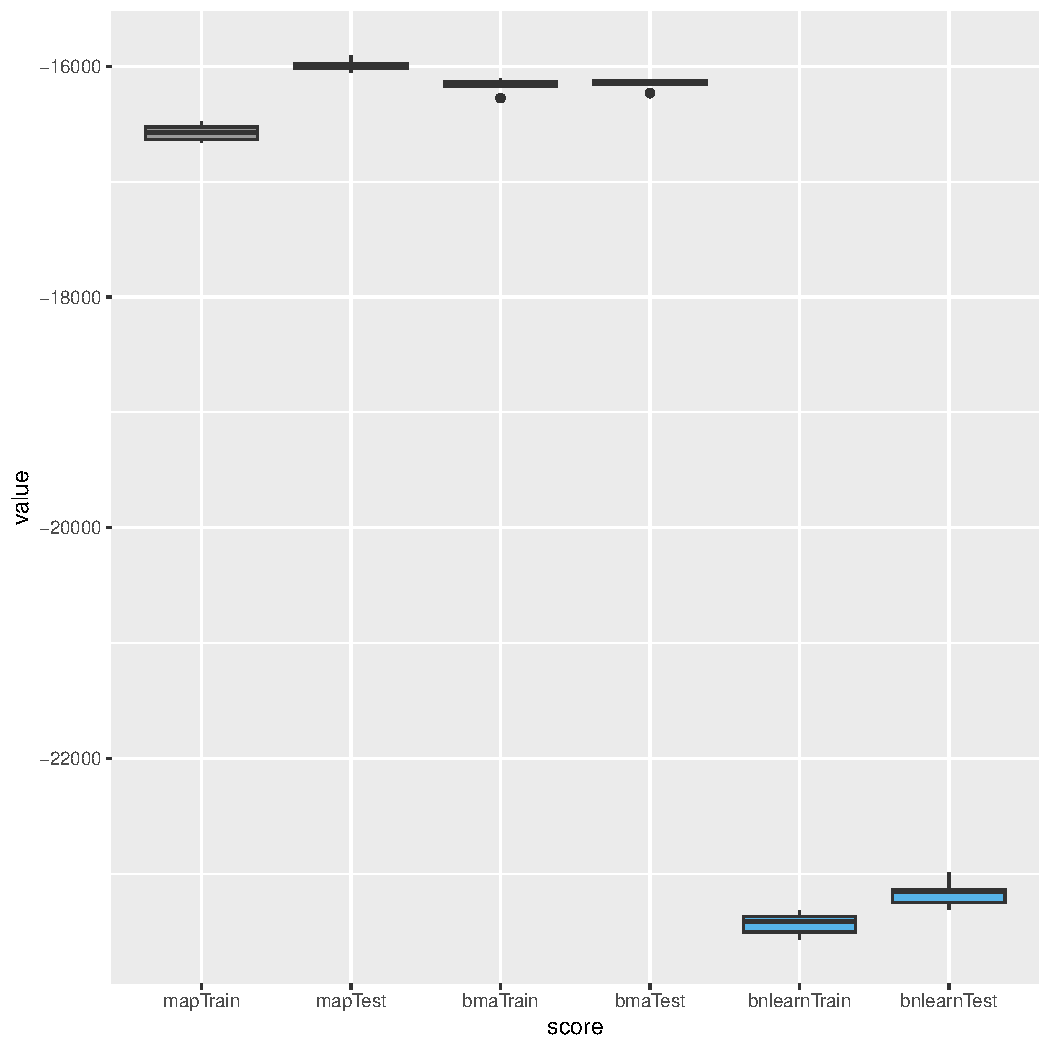
\includegraphics[scale = 0.5]{./figs/win95pts/win95pts-boxplots.pdf}

\subsection{Graphics of evolution}

\begin{tabular}{cc}
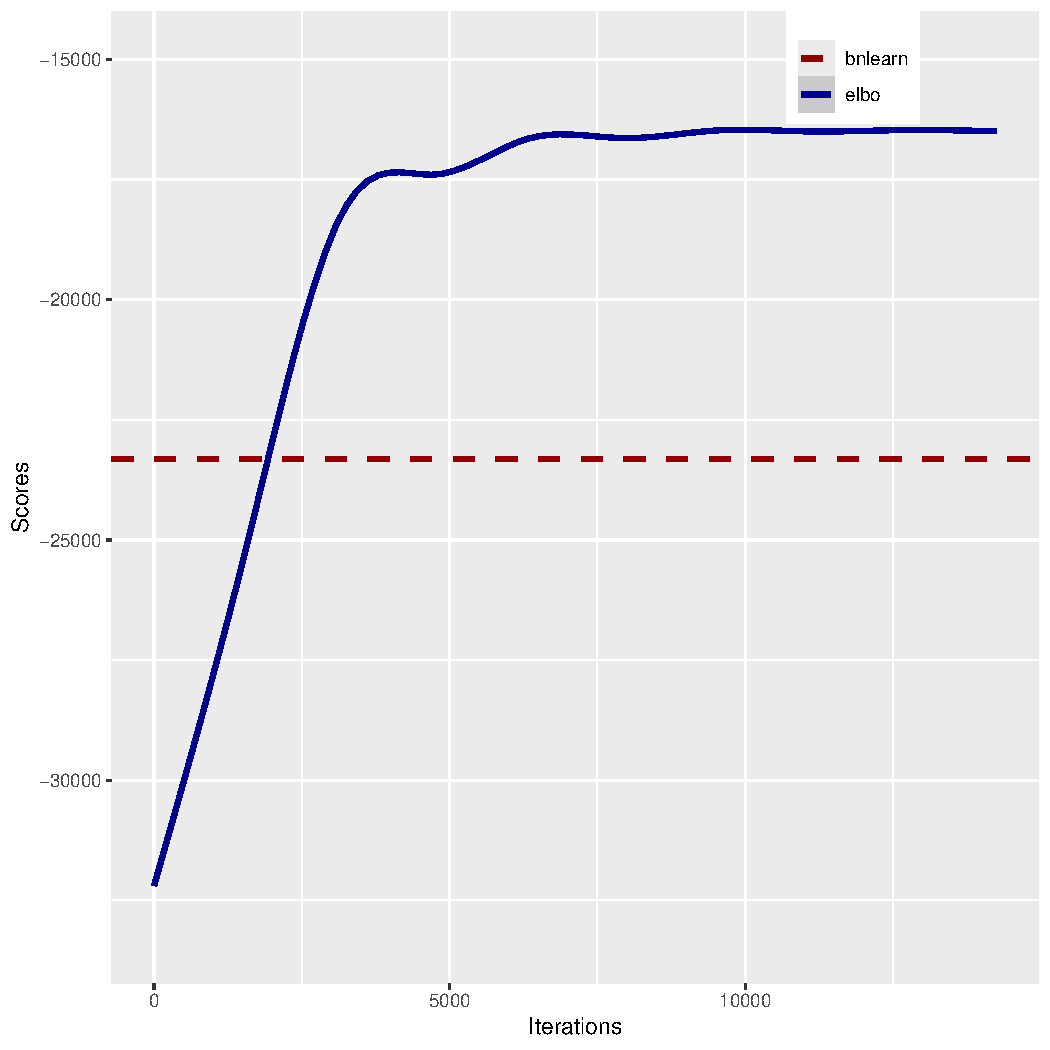
\includegraphics[scale = 0.4]{./figs/win95pts/mapEvolution-1-14252.pdf} &
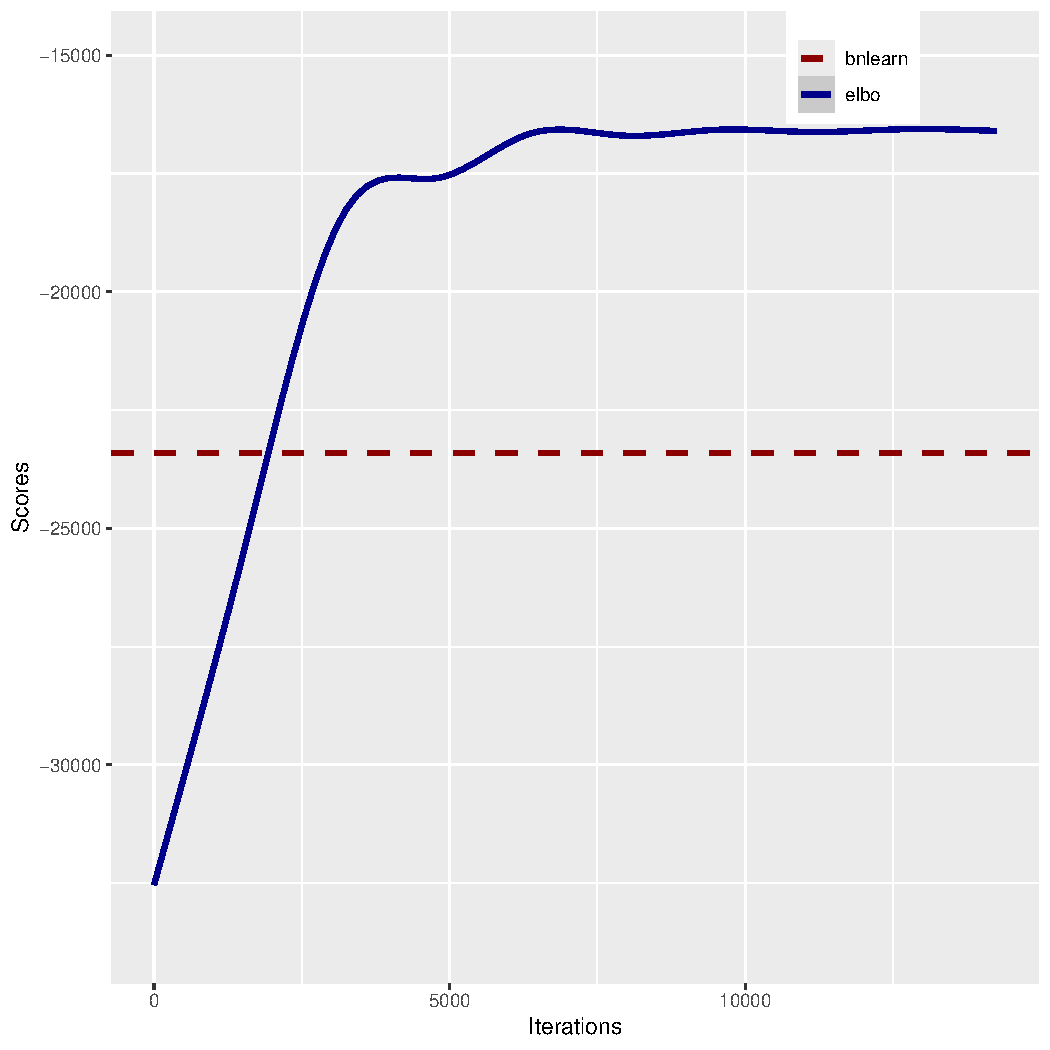
\includegraphics[scale = 0.4]{./figs/win95pts/mapEvolution-2-14252.pdf} \\
\end{tabular}

\begin{tabular}{cc}
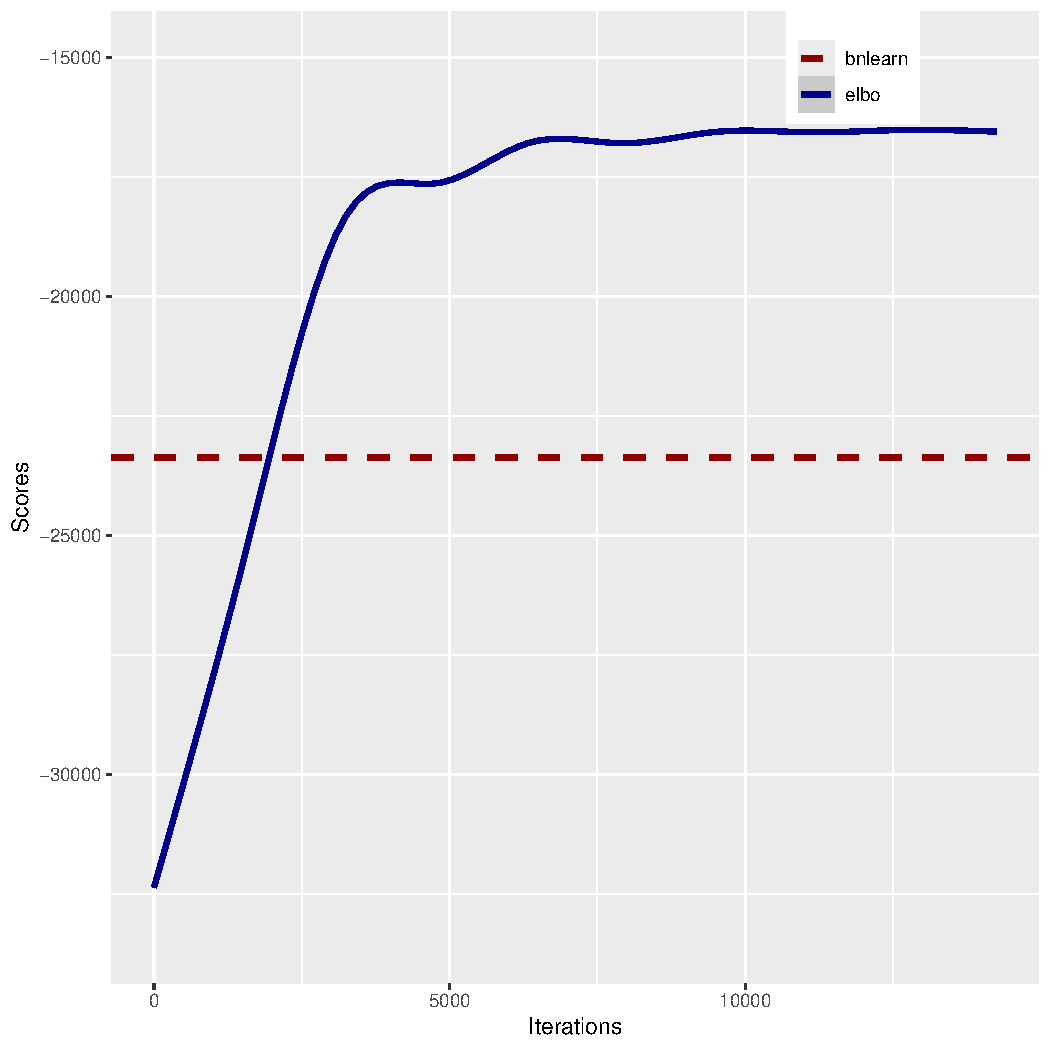
\includegraphics[scale = 0.4]{./figs/win95pts/mapEvolution-3-14252.pdf} &
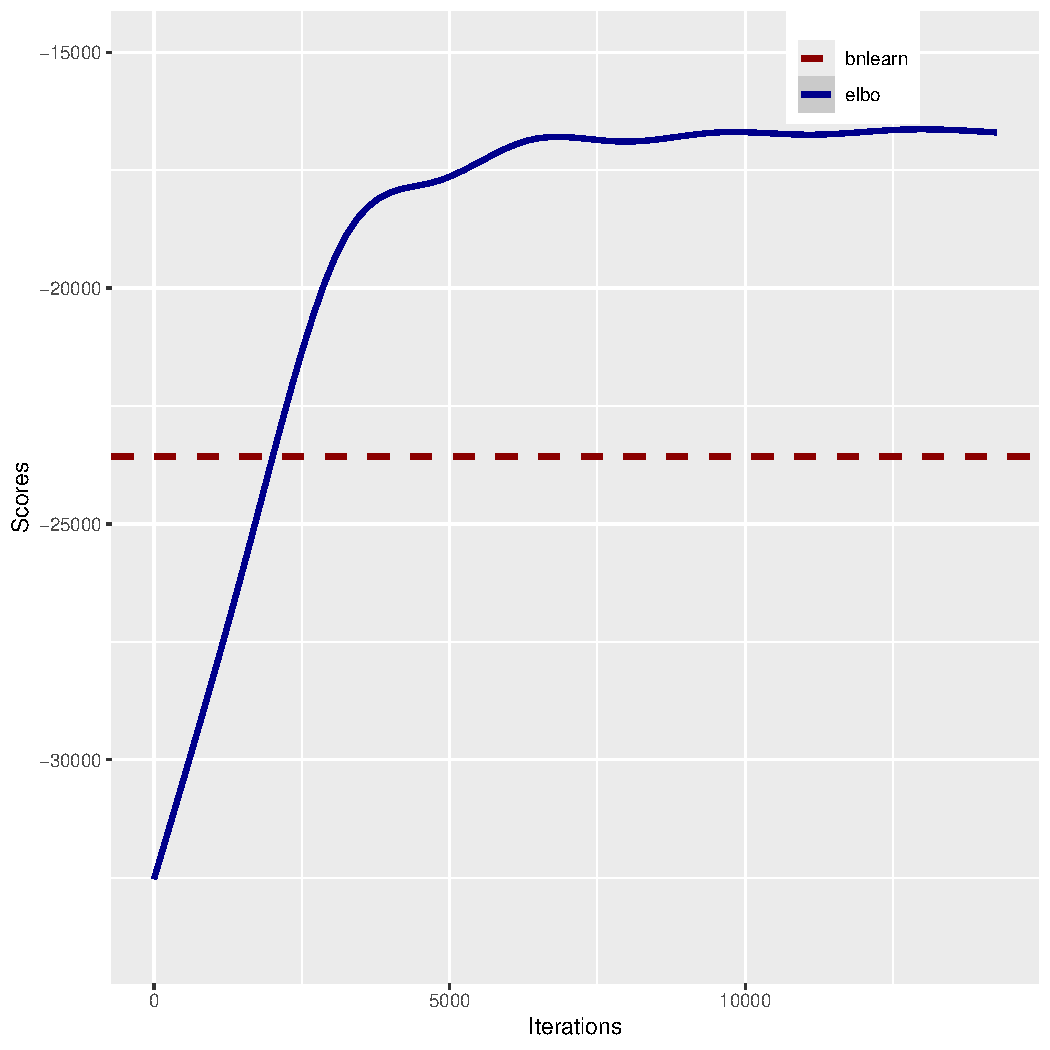
\includegraphics[scale = 0.4]{./figs/win95pts/mapEvolution-4-14252.pdf} \\
\end{tabular}

\begin{tabular}{cc}
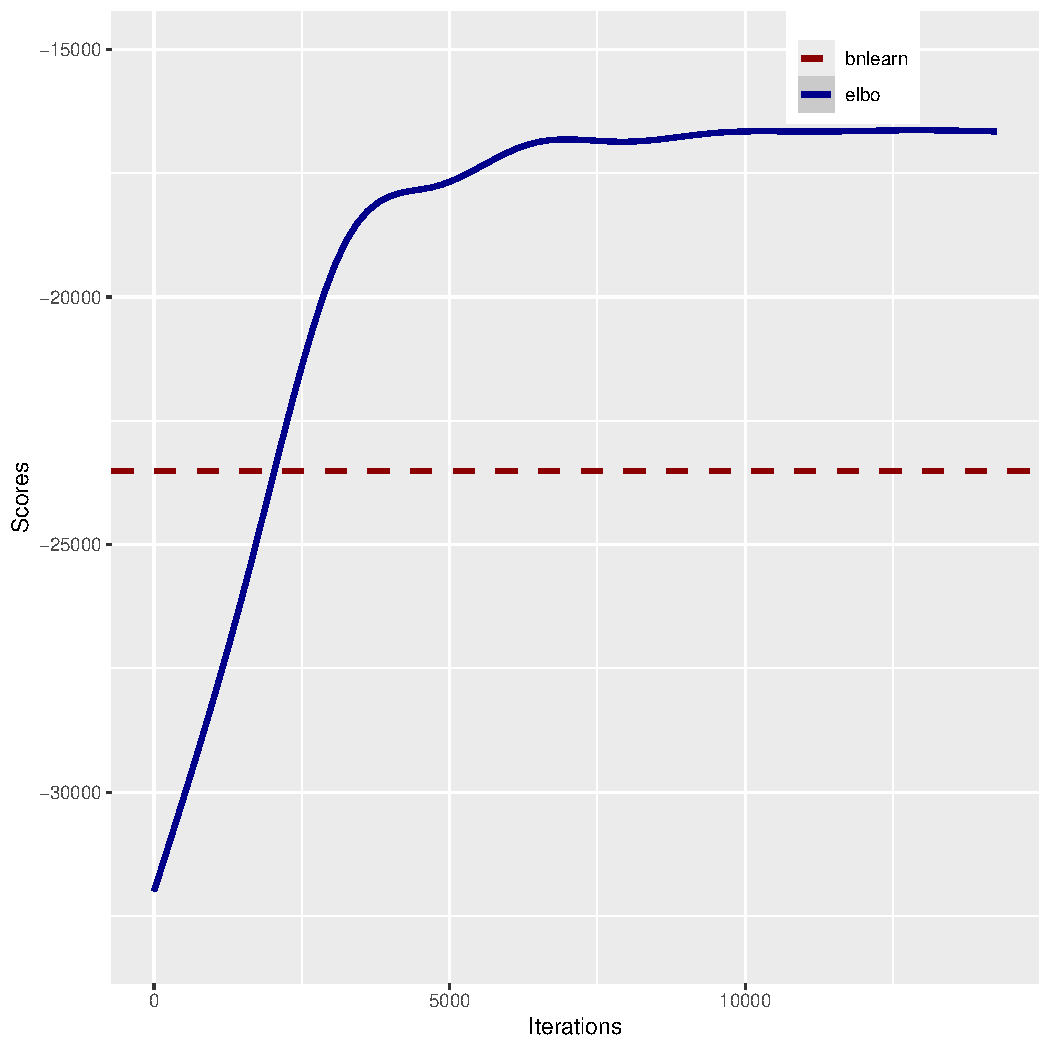
\includegraphics[scale = 0.4]{./figs/win95pts/mapEvolution-5-14252.pdf} &  \\
\end{tabular}

\end{document}
